% Vorlage: https://www.pfsr.de/latex

% -- Anfang Präambel
\documentclass[german,  % Standardmäßig deutsche Eigenarten, englisch -> english
parskip=full,  % Absätze durch Leerzeile trennen
%bibliography=totoc,  % Literatur im Inhaltsverzeichnis (ist unüblich)
%draft,  % TODO: Entwurfsmodus -> entfernen für endgültige Version
]{scrartcl}

\usepackage[utf8]{inputenc}  % Kodierung der Datei
\usepackage[T1]{fontenc}  % Vollen Umfang der Schriftzeichen
\usepackage[ngerman]{babel}  % Sprache auf Deutsch (neue Rechtschreibung)

% Mathematik und Größen
\usepackage{amsmath}
\usepackage[locale=DE,  % deutsche Eigenarten, englisch -> US
separate-uncertainty,  % Unsicherheiten seperat angeben (mit ±)
]{siunitx}
\usepackage{physics}  % Erstellung von Gleichungen vereinfachen

\usepackage{graphicx}  % Bilder einbinden \includegraphics{Pfad/zur/Datei(ohne Dateiendung)}

% Gestaltung
\usepackage{booktabs}  % schönere Tabellen
\usepackage[toc]{multitoc}  % mehrspaltiges Inhaltsverzeichnis
\usepackage{csquotes}  % Anführungszeichen mit \enquote
\usepackage{caption}  % Anpassung der Bildunterschriften, Tabellenüberschriften
\usepackage{subcaption}  % Unterabbildungen, Untertabellen, …
\usepackage{enumitem}  % Listen anpassen
\setlist{itemsep=-10pt}  % Abstände zwischen Listenpunkten verringern

% Manipulation des Seitenstils
\usepackage[headtopline = .5pt]{scrlayer-scrpage}

% Bibliographie
\usepackage[backend=biber]{biblatex}
\addbibresource{bibliography.bib}

% SI-Einheiten darstellen
\usepackage{siunitx}

% Kopf-/Fußzeilen setzen
\pagestyle{scrheadings}  % Stil für die Seite setzen
\clearmainofpairofpagestyles  % Stil zurücksetzen, um ihn neu zu definieren
\automark{section}  % Abschnittsnamen als Seitenbeschriftung verwenden
\ofoot{\pagemark}  % Seitenzahl außen in Fußzeile
\ihead{\headmark}  % Seitenbeschriftung mittig in Kopfzeile

\usepackage[hidelinks]{hyperref}  % Links und weitere PDF-Features

% TODO: Titel und Autor, … festlegen
\newcommand*{\titel}{Weitwinkel-Compton-Koinzidenz-Kalibrierung}
\newcommand*{\autor}{Sebastian Thiede, Alexander Lettau}
\newcommand*{\abk}{WK}
\newcommand*{\betreuer}{V. Melzer}
\newcommand*{\messung}{04.11.2021 \& 11.11.2021}
\newcommand*{\ort}{ASB/406}

\hypersetup{pdfauthor={\autor}, pdftitle={\titel}}  % PDF-Metadaten setzen

% automatischen Titel konfigurieren
\titlehead{Praktikum des IKTP \abk \hfill TU Dresden}
\subject{Versuchsprotokoll}
\title{\titel}
\author{\autor}
\date{\begin{tabular}{ll}
Protokoll: & \today\\
Messung: & \messung\\
Ort: & \ort\\
Betreuer: & \betreuer\end{tabular}}

% -- Ende Präambel

\begin{document}
\begin{titlepage}
\maketitle  % Titel setzen
\tableofcontents  % Inhaltsverzeichnis setzen
\end{titlepage}

% ----- DOKUMENT ANFANG -----

\section{Einführung}
In diesem Praktikumsversuch soll ein Photonendetektor mittels Weitwinkel-Compton-Koinzidenz-Methode (WCKM) kalibriert werden.
Die WCKM ist eine Methode zur Energiekalibrierung von vor allem organischen Szintillatoren. Da organische Szintillatoren Atome mit niedrigen Kernladungszahlen (Niedrig-Z-Szintillatoren) verwenden kann keine Kalibrierung mittels Bestimmung des Vollenergiepeaks stattfinden, denn für die typischerweise verwendeten Kalibrierenergien (\SI{0.5}{\mega\electronvolt} bis \SI{1.5}{\mega\electronvolt}) überwiegt bei niedrigem Z die Compton-Streuung gegenüber dem Photoeffekt.
Für den Versuch wird außerdem ein HPGe-Detektor kalibriert um den Detektor auf Basis des organischen Szintillators mit diesem zu vergleichen. Der HPGe-Detektor kann aufgrund seiner höheren Kernladungszahl mittels Vollenergiepeakanalyse kalibriert werden.

Die zu bearbeitenden Aufgaben sind konkret:
\begin{enumerate}
    \item Vergleich der Detektorspektren
    \item Energiekalibrierung des HPGe-Detektors
    \item Untersuchung einzelner Streuwinkel
    \item Energiekalibrierung des organischen Szintillators
\end{enumerate}

\section{Theorie}

\subsection{organische Szintillatoren}

Szintillatoren sind  Materialien die bei bestrahlung mit energiereichen Photonen oder geladenen Teilchen angeregt werden und die Anregungsenergie in Form von Licht wieder abgeben. Organische Szintillatoren bestehen wie der Name schon vermuten lässt vorwiegend aus Kohlenstoff, Wasserstoff, Sauerstoff und Stickstoff wie es auch in z.B. menschlichem Gewebe der Fall ist. Es liegt daher nahe Detektoren auf Basis organischer Szintillatoren für die Dosismessung im Strahlenschutz zu verwenden. Organische Szintillatoren bestehen typischerweise aus zwei Komponenten: Einem primären Fluoreszenzstoff (z.B. auf Basis von Polyvinyltoluol) und einem \glqq Wellenlängenschieber \grqq{} (z.B. POPOP) da die vom primären Fluoreszenzstoff abgegebenen UV-Strahlen in den meisten durchsichtigen Materialien eine nur sehr geringe Reichweite besitzen.

\subsection{Wechselwirkung von Photonen mit Materie}

Obwohl Photonen in vieler Weise mit Materie wechselwirken können sind für diesen Versuch nur zwei Prozesse von wesentlicher Bedeutung: Die Compton-Streuung und der Photoeffekt. In den folgenden Abschnitten werden beide näher erläutert.

\subsubsection{Photoeffekt}

Der Photoeffekt beschreibt die Anregung von Elektronen durch Absorption eines Photons.
Für den HPGe-Detektor ist vor allem der innere photoelektrische Effekt von Bedeutung. Er beschreibt die Zunahme der Leitfähigkeit eines Halbleiters durch Bildung von nicht aneinander gebundenen Elektron-Loch-Paaren. Der HPGe-Detektor besteht aus einem hochreinen Germanium-Kristall der zwischen einem $n^{+}$ Kontakt (typ. durch Lithium-eindiffusion) am positiven Spannungspol und einem $p^{+}$ Kontakt (typ. durch Bor-implantation) am negativen Spannungspol sitzt; Der Detektor insgesamt entspricht einer Halbleiterdiode in Sperrichtung. Trifft ein Photon auf den Detektor und erzeugt ein Elektron-Loch-Paar werden durch die anliegende Spannung Elektron und Loch abgesaugt und bilden so einen detektierbaren Verschiebungsstrom. Dafür muss das einfallende Photon natürlich genügend Energie besitzen um die Bandlücke zu überwinden (Für Germanium \SI{0.67}{\electronvolt}), praktisch jedoch deutlich mehr um das Siganl-Rausch-Verhältnis groß genug zu bekommen. So werden bei einfallenden Photonen von \SI{1}{\mega\electronvolt} etwa \num{3e5} Elektron-Loch-Paare erzeugt \cite{HPGe-Detektor}. Da bei Raumtemperatur eine ständige thermische Anregung der Elektronen enormes Signalrauschen verursachen würde ist eine Abkühlung mit flüssigem Stickstoff notwendig.
Für den zu kalibrierenden Detektor ist vor allem der äußere photoelektrische Effekt von Bedeutung, genauer für den Photoelektronenvervielfacher (Abb. \ref{theorie_PEV}).

\begin{figure}[ht]
	\centering
  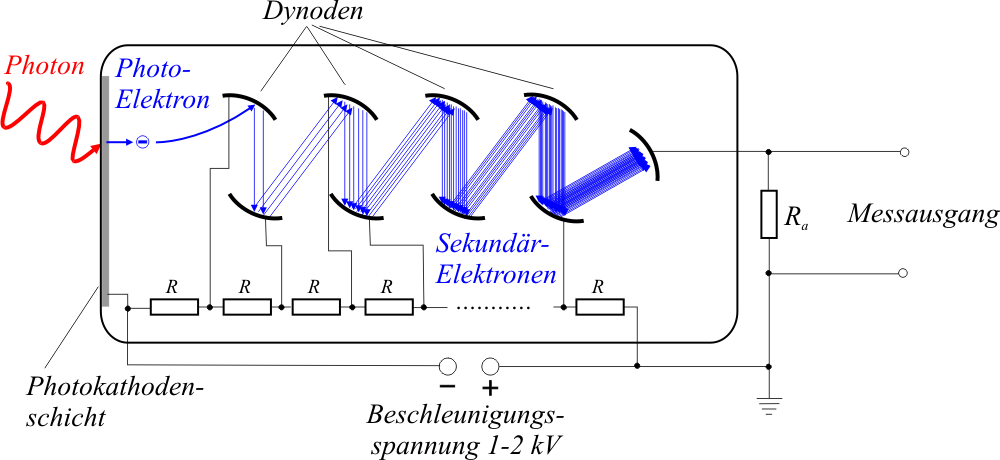
\includegraphics[width=0.85\textwidth]{images/Photomultiplier_schema_de.png}
	\caption{Schematik Photoelektronenvervielfacher}
	\label{theorie_PEV}
\end{figure}

Dort werden durch das Szintillationsphoton Elektronen aus einer Photokathode ausgeschlagen, durch angelegte Spannung zur ersten Dynode beschleunigt wo sie mit der gewonnenen kinetischen Energie weitere Elektronen auschlagen. Dieser Prozess wird einige male wiederholt bis ein messbarer elektrischer Impuls an der Anode entstehen kann.

\subsubsection{Compton-Streuung}

\subsection{Weitwinkel-Compton-Koinzidenz-Methode}

\section{Kalibrierung des Szintillators}

\subsection{Vergleich der Detektorspektren}

Im ersten Schritt wurden die Spektren mehrerer Quellen für den Szintillator, wie auch den Ge-Detektor, aufgenommen und die Ergebnisse verglichen.
Genutzt wurden hierfür eine $^{22}$Na- und eine $^{133}$Ba-Probe, welche auf den HPGe-Detektor und neben den Szintillator gelegt wurden.
Die Messzeit betrug für $^{22}$Na \SI{5}{\minute} und für $^{133}$Ba \SI{4}{\minute}.
Eine Messung der Untergrundstrahlung wurde nicht durchgeführt, da sie für den einfachen Vergleich zweier Spektren auch nicht notwendig wäre.
Wie in Abb. \ref{NaGe} und \ref{NaSzin} zu sehen ist, war die Aktivität der $^{22}$Na Probe recht niedrig.
Im Ge-Spektrum lässt sich prinzipiell ein stark ausgeprägter Peak, zwischen den Kanälen 500 und 600, erkennen, das Compton-Kontinuum ist jedoch recht verschwommen.
Das Szintillator-Spektrum wiederum scheint hier unbrauchbar.
Es lässt sich nur ungefähr der Bereich des Comtpon-Kontinuums erahnen.
Eine Kalibrierung mithilfe dieser Probe sollte nur schwer möglich sein, da für den Ge-Detektor mehrere Peaks notwendig wären und das Szintillator-Spektrum einfach zu schwach ausgeprägt ist.
Prinzipiell könnten die Spektren mit einer längeren Messzeit verbessert werden, in diesem Versuch standen jedoch mehrere Proben zur Auswahl, weshalb dies nicht gemacht wurde.

\begin{figure}[h]
\minipage{0.5\textwidth}
  \includegraphics[width=\linewidth]{images/Na22ge.png}
  \caption{Ge-Detektor}
  \label{NaGe}
\endminipage\hfill
\minipage{0.5\textwidth}
  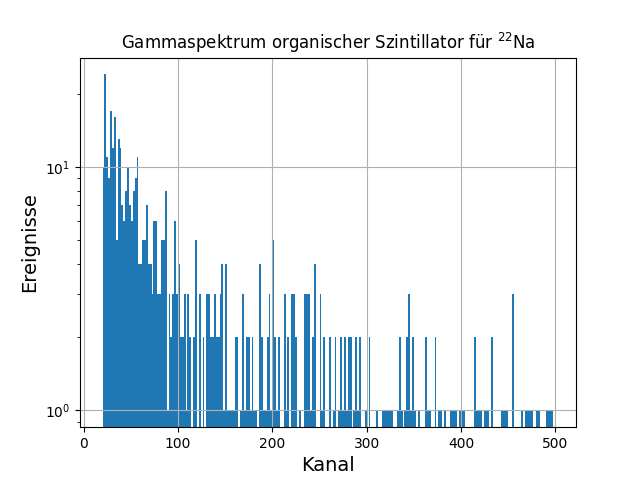
\includegraphics[width=\linewidth]{images/Na22szin.png}
  \caption{Szintillator}
  \label{NaSzin}
\endminipage\hfill
\end{figure}

Die $^{133}$Ba Probe besaß eine im Vergleich dazu deutlich stärkere Aktivität, was sich positiv auf die Spektren (Abbildungen \ref{BaGe} und \ref{BaSzin}) ausgewirkt hat.
Im Spektrum des Ge-Detektors lassen sich jetzt mehrere Peaks deutlich erkennen.
Eine Kalibirierung anhand dieser sollte jetzt möglich sein.
Das Szintillator-Spektrum dieser Probe wird, wie  zu erwarten war, vom Compton-Kontinuum dominiert.
Die Compton-Kante ist hierbei schwach ausgeprägt, was eine herkömmliche Kalibrierung, wieder wie zu erwarten, erschweren würde.
Eine längere Messzeit oder Beseitigung der Untergrundstrahlung würde hier zwar helfen, aber die erreichbaren Genauigkeiten bei der Kalibrierung mit dem Rückstreupeak oder Compton-Kante allein sind für eine Anwendung nicht ausreichend.
Aufällig ist außerdem ein recht stark ausgeprägter Peak im niederenergetischen Bereich (ungefähr bei Kanal 50).
Hierbei könnte es sich um einen stark ausgeprägten Rückstreupeak handeln.
Aufgrund der besseren Spektren wird im folgenden die $^{133}$Ba-Probe genutzt.

\begin{figure}[h]
\minipage{0.5\textwidth}
  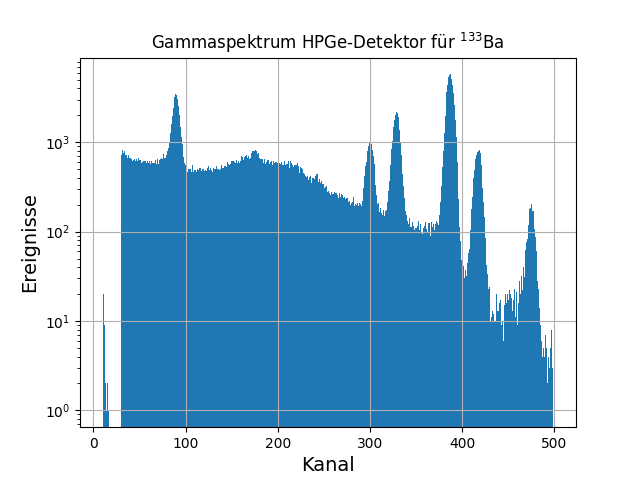
\includegraphics[width=\linewidth]{images/ba133Ge.png}
  \caption{Ge-Detektor}
  \label{BaGe}
\endminipage\hfill
\minipage{0.5\textwidth}
  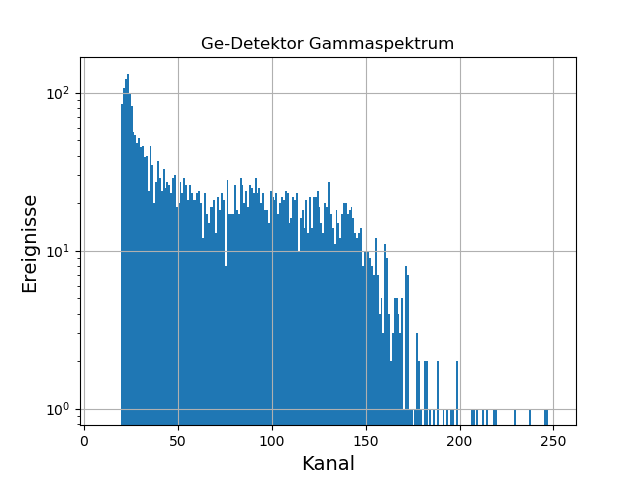
\includegraphics[width=\linewidth]{images/ba133Szin.png}
  \caption{Szintillator}
  \label{BaSzin}
\endminipage\hfill
\end{figure}

\subsection{Energiekalibrierung des Ge-Detektors}

Ausgehend vom aufgenommenen Spektrum wird im folgenden eine Energiekalibrierung des Ge-Detektors mittels einer Vollenergiepeak-Analyse durchgeführt.
Dafür ist es als erstes notwendig, die sichtbaren Peaks zu identifizieren.
Dies wurde durch Vergleiche mit bekannten Nuklid-Karten (z.B. \cite{IAEA}) realisiert.
Die Ergebnisse sind in Abb. \ref{GeKali} zu sehen.
Eine Identifikation der Peaks mittels der häufigsten Gammazerfälle von $^{133}$Ba war möglich.
Zusätzlich zu diesen fällt jedoch ein weiterer Peak mit relativ geringer Intensität um Kanal 480 herum auf.
Ein entsprechender Gammazerfall von $^{133}$Ba ist nicht in \cite{IAEA} zu finden.
Daher sollte es sich hier um Untergrundstrahlung von einem natürlichen Nuklid handeln.
Eine Identifkation von diesem könnte erfolgen, aufgrund der relativ geringen Intensität und der foldendermaßen hohen statistischen Ungenauigkeit wurde dies jedoch nicht getan und der Peak nicht für die Kalibrierung genutzt.

\begin{figure}[h]
  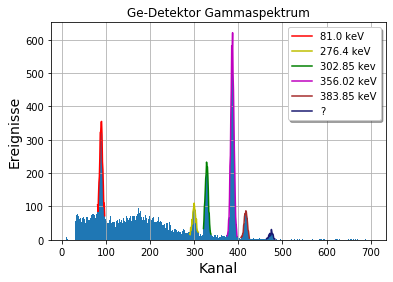
\includegraphics[width=\linewidth]{images/ba133Kali.png}
  \caption{Vollenergiepeakanalyse des Ge-Detektors mit $^{133}$Ba Spektrum}
  \label{GeKali}
\end{figure}

Die entsprechenden Peaks wurden mit einer Gaussfunktionen entsprechend
\begin{equation}
N(K) = a \cdot \exp \left( - \frac{(K - K_{0})^{2}}{2 \sigma ^{2}} \right)
\end{equation}
gefittet, um Mittelwerte $\mu$ und Standardabweichungen $\sigma$ dieser zu bestimmen.
In der Gaussfunktion dient $a$ als Normierungsfaktor, der für die weitere Betrachtung keine Rolle spielt.
Die Ergebnisse sind in Tabelle \ref{peaks} zusammengefasst.
Hier fällt auf, dass die Standardabweichungen der Peaks recht konstant sind.

\begin{table}[h]
\centering
\begin{tabular}{|c | c |c |}
\hline
$E_{\gamma}$ [\si{\kilo\electronvolt}]  & $\mu$ & $\sigma$ \\
\hline
81.00 & 89.0 & 3.1 \\
276.40 & 299.9 & 3.6 \\
302.89 & 328.4 & 3.7 \\
356.02 & 386.4 & 3.7 \\
383.85 & 416.8 & 3.7 \\
\hline
\end{tabular}
\caption{Gaussfit der Peaks}
\label{peaks}
\end{table}

Aus den Mittelwerten wird der Kanal, welcher mit der Zerfallsenergie korrespondiert bestimmt, indem der Mittelwert $\mu$ zur nächsten natürlichen Zahl K gerundet wird.
Als Maß für die Unsicherheit der Energiebestimmung wird die mittlere Halbwertsbreite (FWHM), ebenfalls auf natürliche Zahlen gerundet, genutzt.
Diese ist defininiert als Breite der Gaussfunktion bei halber Höhe und dient uns als Unsicherheit der Energiebestimmung.
Sie berechnet sich aus der Standardabweichung $\sigma$ mit:
\begin{equation}
\text{FWHM} = 2 \sqrt{2 \ln{2}} \cdot \sigma
\end{equation}
Die Ergebnisse sind in Tab. \ref{kanal} zusammengefasst.

\begin{table}[h]
\centering
\begin{tabular}{|c | c |c |}
\hline
$E_{\gamma}$ [\si{\kilo\electronvolt}]  & $K_{\gamma}$ & FWHM \\
\hline
81.00 & 89 & 7 \\
276.40 & 300 & 8 \\
302.89 & 328 & 9 \\
356.02 & 386 & 9 \\
383.85 & 417 & 9 \\
\hline
\end{tabular}
\caption{Bestimmung der Kanäle}
\label{kanal}
\end{table}

Mit Kentnis der fünf Energiepeaks sowie der korrespondierenden Kanäle ist jetzt die Bestimmung einer Kalibriergerade des Ge-Detektors möglich.
Dafür wurden die Energien über die Kanäle geplottet und eine lineare gefittet.
Das Ergebnis davon ist in \ref{Gegerade} zu sehen.
Dieser Fit wurde mithilfe des in \cite{Fit_bivariate} beschriebenen Algorithmus nach York durchgeführt, wobei für die Fehler in der Energie extrem kleine Werte angenommen wurden (da die Photonenenergien sehr gut bekannt sind), sodass diese keinen Einfluss auf das Ergebnis haben.
Damit ergibt sich die Kalibrierung des HPGe-Detektors:
\begin{gather}
    E_{\text{HPGe-Detektor}} (K) = [(0.925 \pm 0.028) \cdot K + (-1.155 \pm 8.678)] \ \si{\kilo\electronvolt}
\end{gather}
Es sollte erwähnt werden, dass die scheinbar große Unsicherheit des Schnittpunktes mit der y-Achse von $8.678$ in anbetracht der FWHM der Gaussfits sinnvoll erscheinen.
Schaut man sich die Kalibriergerade an so sieht man, dass beim parallelverschieben der Fitgerade zu den Rändern des Fehlerbereichs durchaus eine Unsicherheit in dieser Größenordnung für den Schnittpunkt mit der y-Achse entstehen kann.
Diese Unsicherheit entspringen also nahezu ausschließlich aus dem FWHM.
Da die Punkte alle sichtlich gut auf einer geraden liegen, ist der Fehler des Anstiegs klein (Relativfehler etwa \SI{3}{\percent}).
Daher liegt auch der Zahlenwert der Unsicherheit des Schnittpunktes mit der y-Achse von $8.678$ so nahe am durchschnittlichen Wert der oben genannten FWHM ($8.4$).
Physikalische oder technische Ungenauigkeiten, wie z. B. die Untergrundstrahlung, wurden hier nicht betrachtet.

\begin{figure}[h!]
  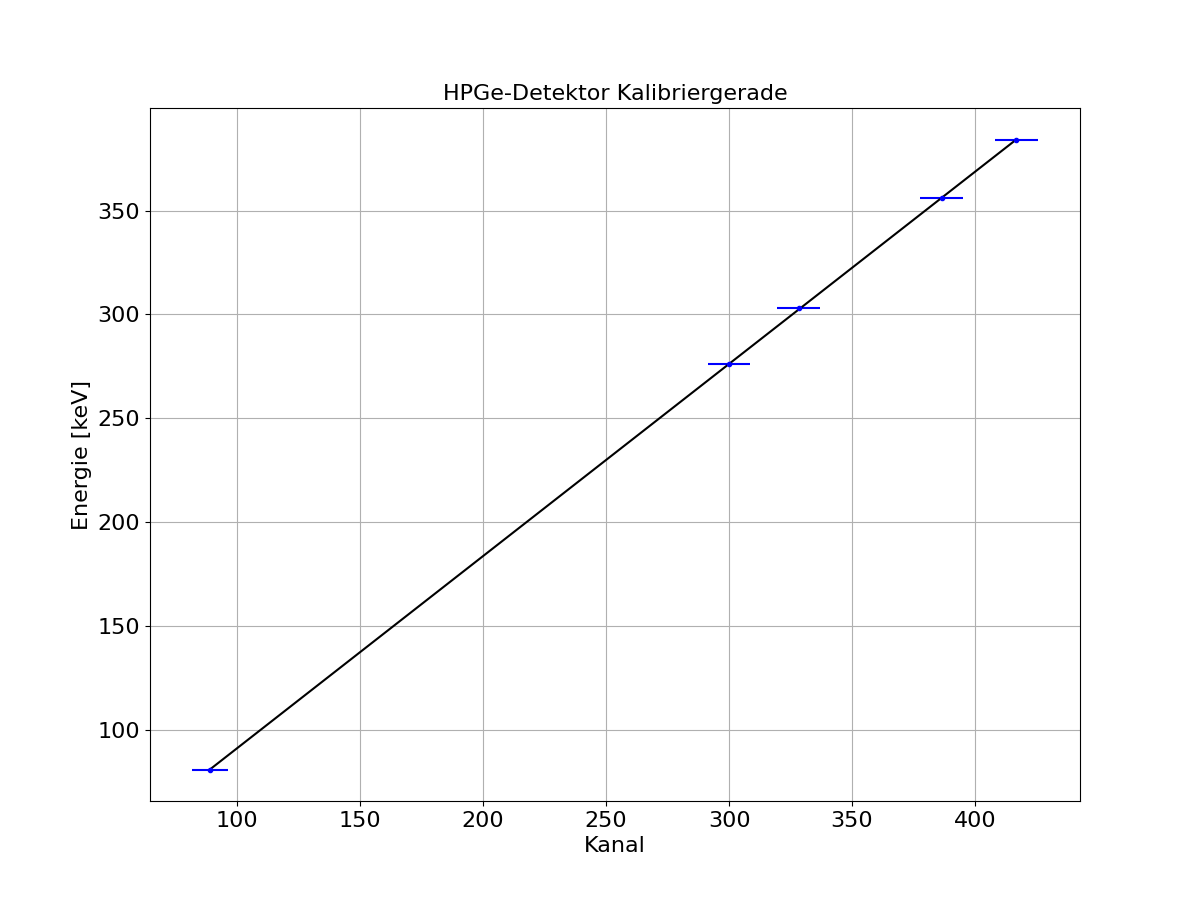
\includegraphics[width=\linewidth]{images/Kalibriergerade1.png}
  \caption{Kalibriergerade des Ge-Detektors}
  \label{Gegerade}
\end{figure}

\subsection{Untersuchung einzelner Streuwinkel}

Zur Kalibrierung des organischen Szintillators wurde die WCKM verwendet. Dafür wurden immer koinzidente Ereignisse aufgenommen und die gemessenen Detektorkanäle in einem zweidimensionalen Histogramm gegeneinander Aufgetragen. Vor der eigentlichen Kalibrierung wurden jedoch einzelne Streuwinkel untersucht. Dafür wurde die $^{22}$Na Probe mithilfe des Roboterarms an verschiedene Koordinaten gefahren (s. Tabelle \ref{kali_szint_coords}). Die entsprechenden Histogramme sind in Abbildung \ref{kali_szint_winkelabh} zu sehen.

\begin{table}[h]
    \centering
    \begin{tabular}{|c | c |c |}
        \hline
        Koordinaten $(x,y,z)$  & Streuwinkel & Messzeit \\
        \hline
        $(-33, 10, 7)$ & \SI{70.7}{\degree} & \SI{60}{\minute} \\
        $(-33, 4, 15)$ & \SI{60.0}{\degree} & \SI{30}{\minute} \\
        $(-33, 6, 20)$ & \SI{50.2}{\degree} & \SI{30}{\minute} \\
        $(-33, 9, 24)$ & \SI{41.2}{\degree} & \SI{30}{\minute} \\
        $(-33, 20, 27)$ & \SI{20.3}{\degree} & \SI{30}{\minute} \\
        \hline
    \end{tabular}
    \caption{Angefahrene Koordinaten der $^{22}$Na Probe, daraus resultierender Streuwinkel (grob) und Messzeit an dem jeweiligen Punkt}
    \label{kali_szint_coords}
\end{table}

\begin{figure}[ht]
	\centering
    \begin{tabular}{c c}
        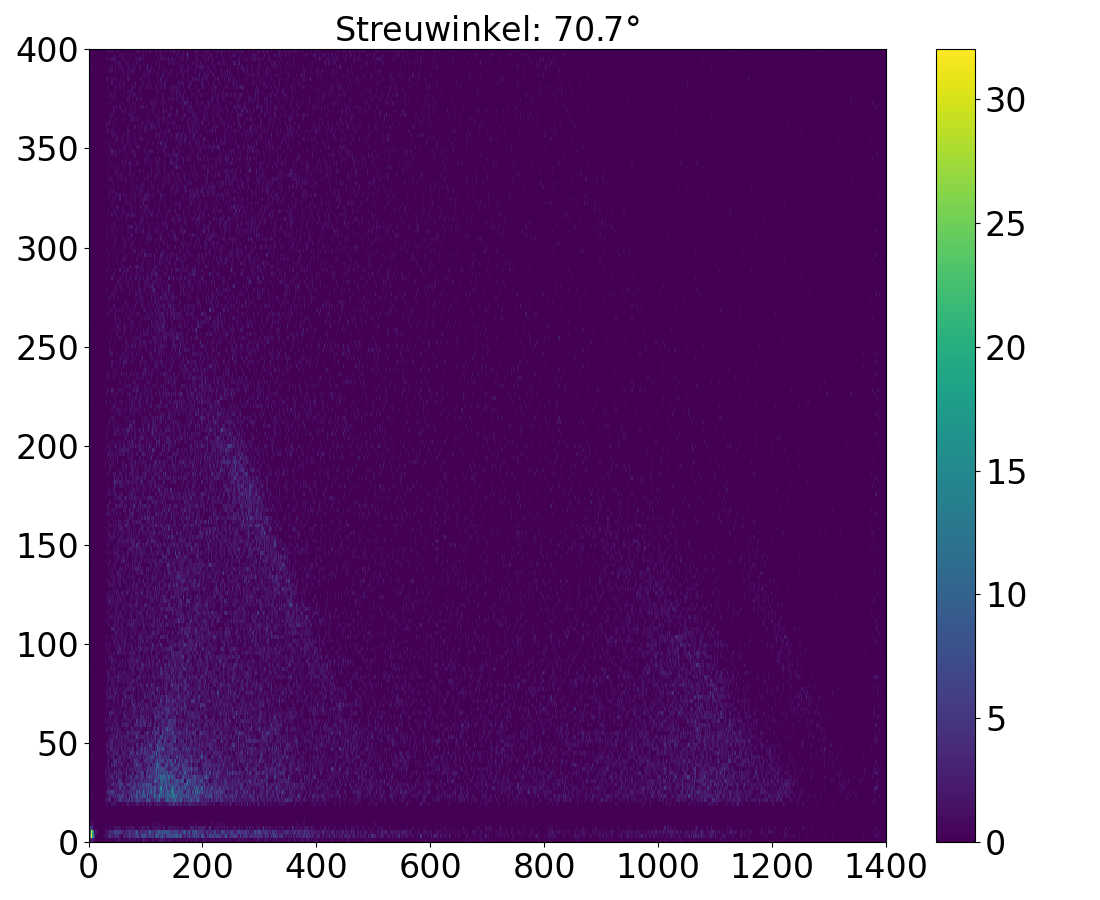
\includegraphics[width=0.49\textwidth]{images/kali_szint_Streuwinkel_70.png} & 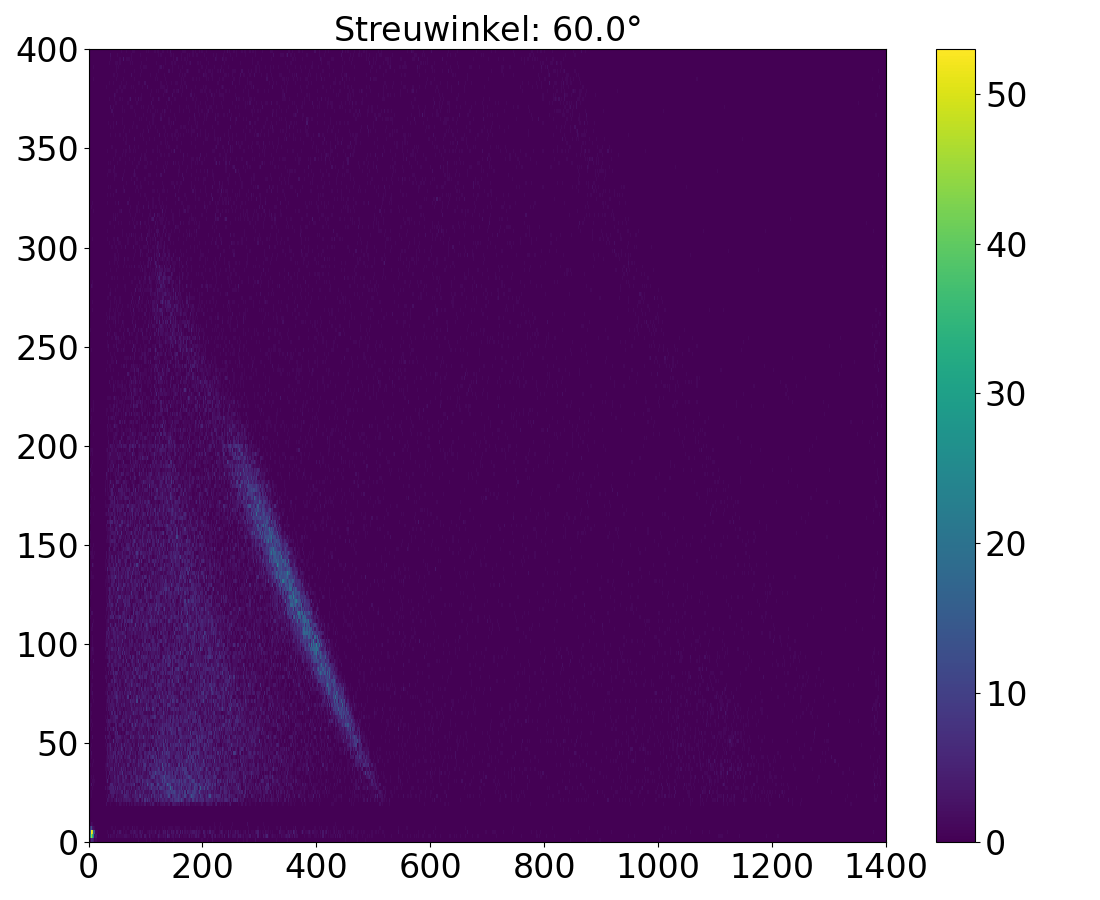
\includegraphics[width=0.49\textwidth]{images/kali_szint_Streuwinkel_60.png} \\ 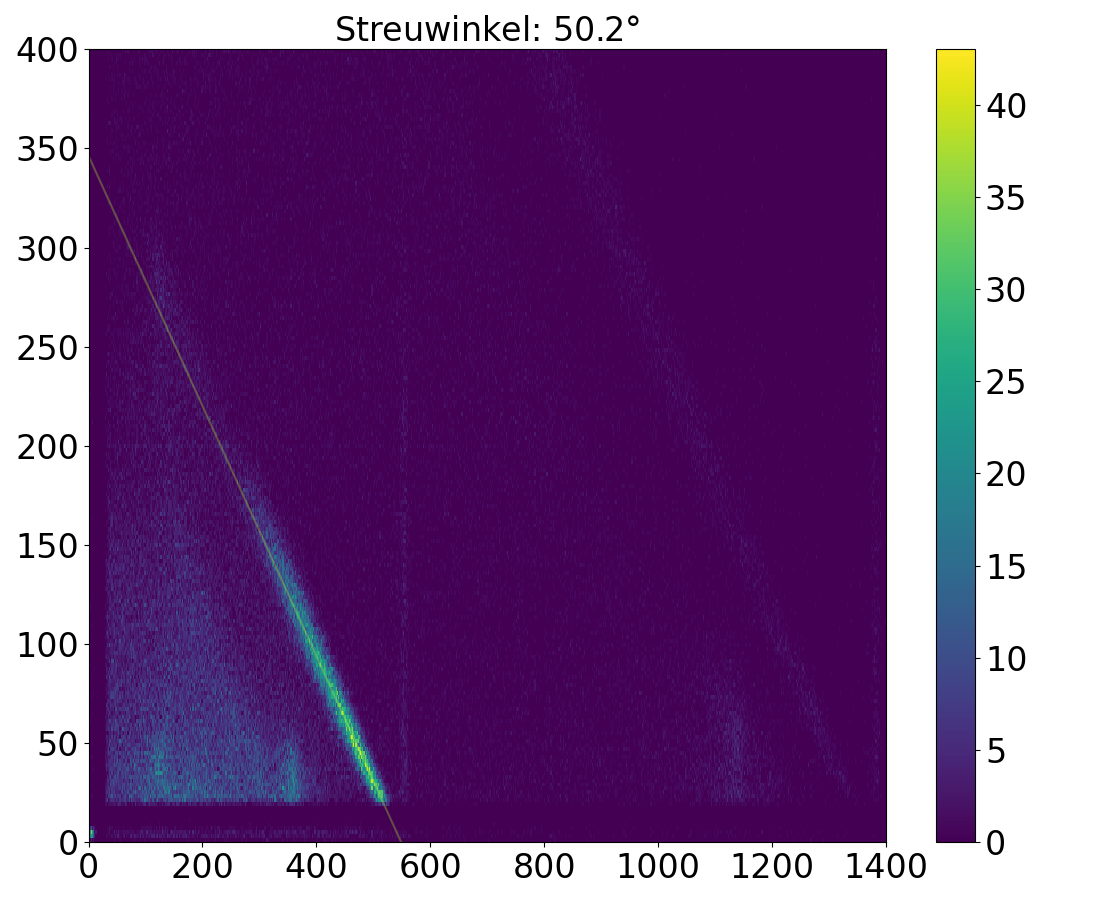
\includegraphics[width=0.49\textwidth]{images/kali_szint_Streuwinkel_50.png} & 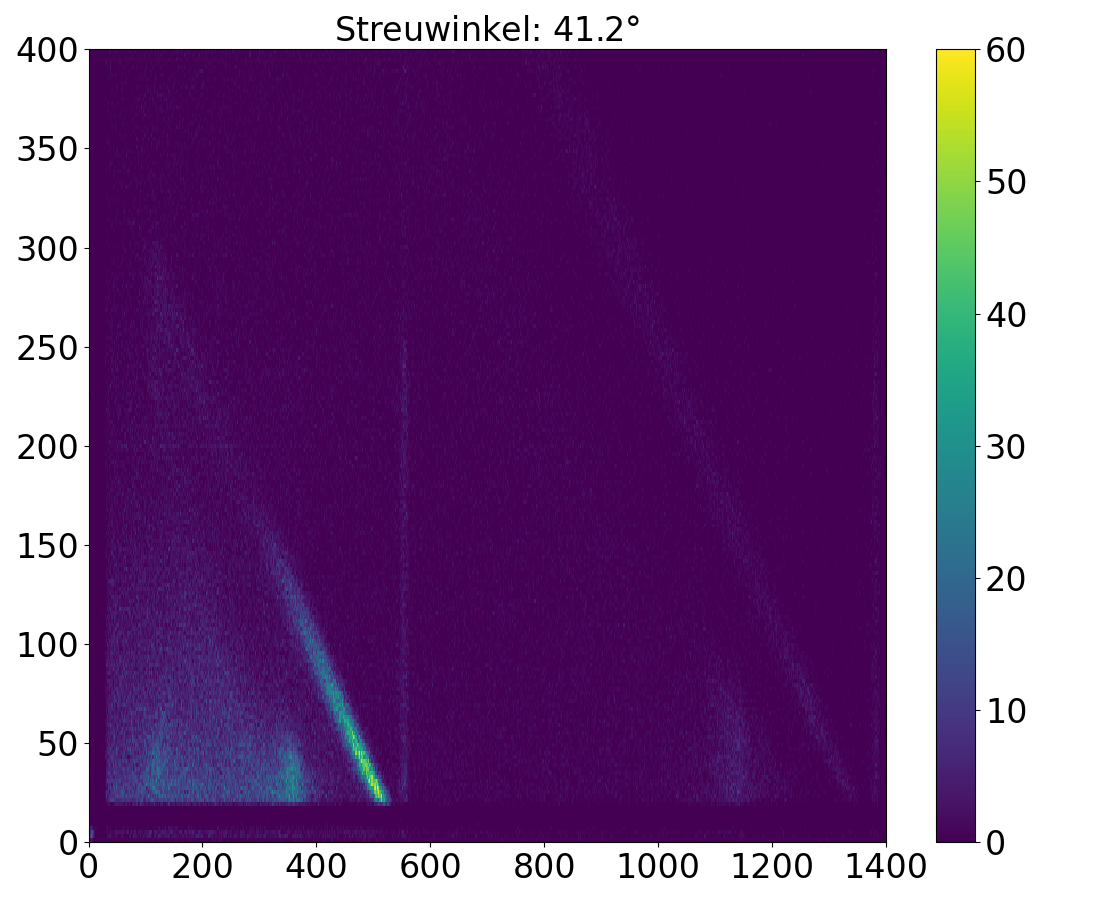
\includegraphics[width=0.49\textwidth]{images/kali_szint_Streuwinkel_40.png} \\\
        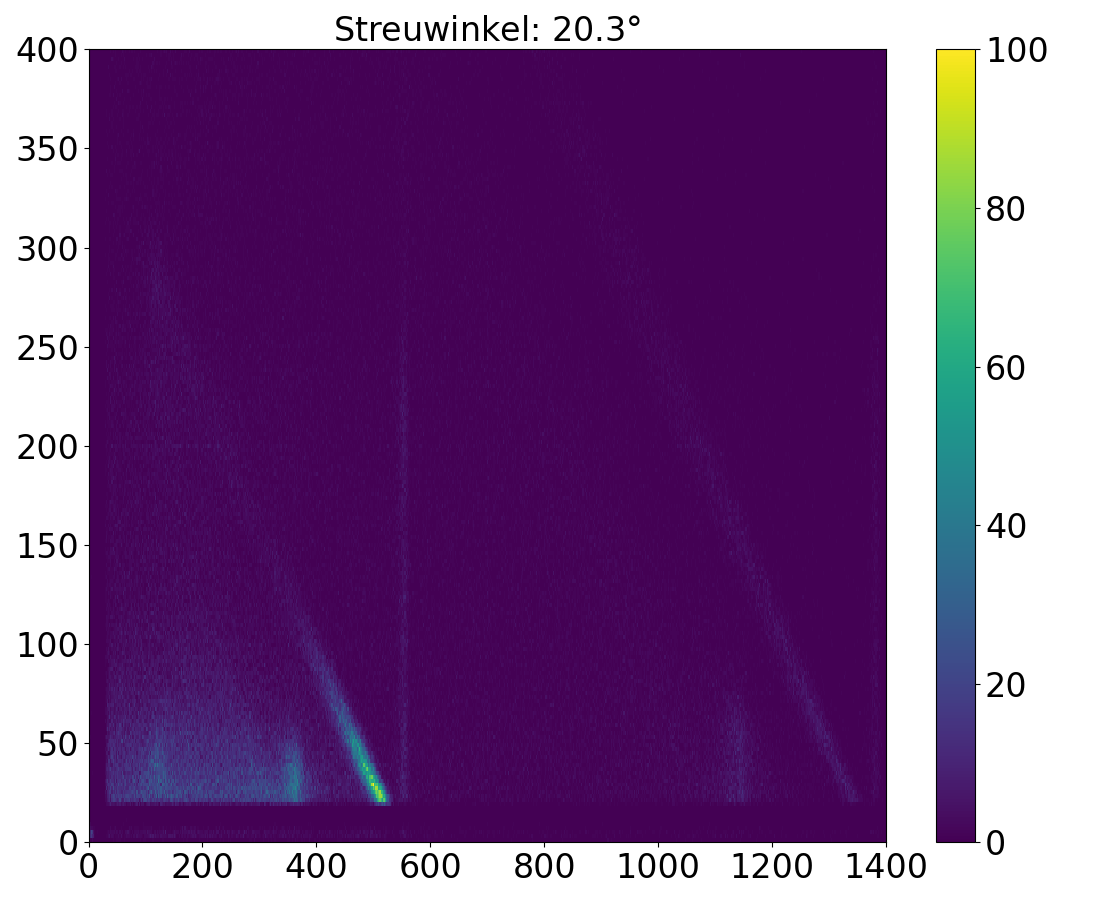
\includegraphics[width=0.49\textwidth]{images/kali_szint_Streuwinkel_20.png} & \\
    \end{tabular}
	\caption{Histogramme der koinzidenten Ereignisse für verschiedene Streuwinkel im Szintillator bei nutzung einer $^{22}$Na Probe, für den Streuwinkel von \SI{50.2}{\degree} ist die gesuchte lineare Beziehung der Detektorkanäle bei koinzidenten Ereignissen eingetragen}
	\label{kali_szint_winkelabh}
\end{figure}

Man erkennt in diesen Histogrammen einige Dinge. Zum ersten verschiebt sich mit sinkendem Streuwinkel der Bereich in dem besonders viele Ereignisse auftreten zu höheren Kanälen im HPGe-Detektor und zu niedrigeren im Szintillationsdetektor. Auch sieht man sofort den linearen Zusammenhang der gemessenen Kanäle (Energien). Diesen kann man beobachten für jede von der Strahlungsquelle abgegebene Energie der Photonen, jedoch ist die im Bild rechte Gerade deutlich schwerer zu erkennen. Man kan daraus folgern das wie bereits diskutiert bei koinzidenten Ereignissen häufig die Energie die bei einer Compton-Streuung nicht im Szintillator deponiert wird im HPGe-Detektor deponiert wird. Man kann anhand der Intensitäten der Punkte auf der Geraden (siehe Farbskala) außerdem darauf schließen, dass ein Streuen in kleineren Winkeln wahrscheinlicher ist und damit in der selben Messzeit öfter auftritt. Man muss dazu erwähnen das für den Streuwinkel von \SI{70.7}{\degree} eine Bleiverschirmung zwischen Quelle und Szintillator stand womit dieses Histogramm für diese Aussage nicht herangezogen werden kann.

\subsection{Energiekalibrierung des organischen Szintilators}

Für die Kalibrierung wurden die diagonalen, linearen Bereiche gefittet und dann der Schnittpunkt der Geraden mit der y-Achse gesucht. Dies entspräche dann nämlich dem Fall das die im HPGe-Detektor deponierte Energie $0$ ist und sämtliche Energie des Photons im Szintillator deponiert wurde. Ein Beispiel für einen Fit ist in Abb. \ref{kali_szint_bsp_fit} zu sehen.

\begin{figure}[ht]
	\centering
    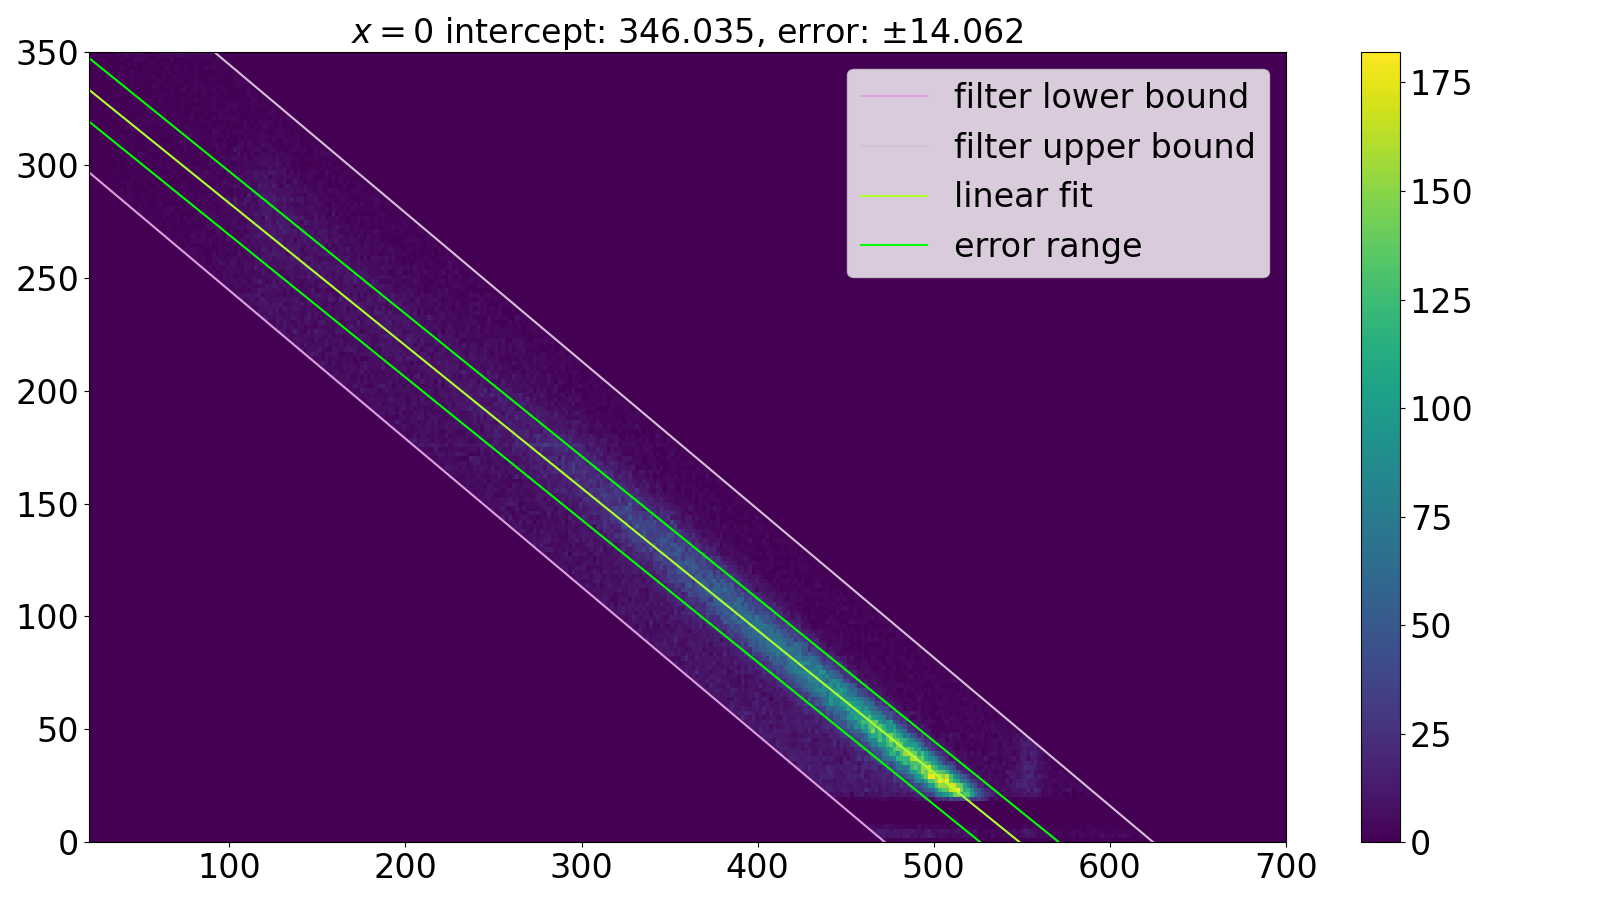
\includegraphics[width=0.98\textwidth]{images/kali_szint_fit_Na22.png}
	\caption{Beispiel für die verwendete Prozedur der linearen Regression für Nutzung einer $^{22}$Na Probe. Zuerst wurde der grobe Bereich des linearen Zusammenhangs ausgeschnitten. Danach wurde eine lineare Regression der Daten durchgeführt. Zuletzt wurden zwei Geraden äquidistant und parallel zur Regressionsgeraden verschoben bis $ 68 \% $ ($1 \sigma$) aller Punkte des ausgeschnittenen Bereichs innerhalb dieser Geraden liegen. Die Schnittpunkte dieser Geraden mit der y-Achse stellen unsere Messunsicherheit dar.}
	\label{kali_szint_bsp_fit}
\end{figure}

Bei der Kalibrierung mit $^{22}$Na wurden die Daten der Streuwinkelmessung und eine zweistündige Messung bei der die Probe in einem Kreisbogen gefahren wurde benutzt. Bei der Kalibrierung mit $^{133}$Ba wurde die Probe \SI{4.5}{\hour} im Kreisbogen um den Szintillator gefahren. Die Ergebnisse des Fittings sind in Tabelle \ref{kali_szint_Energien} zu sehen.

\begin{table}[h]
    \centering
    \begin{tabular}{|c | c | c | c|}
        \hline
        Element & Photonenenergie & Kanal & Unsicherheit im Kanal \\
        \hline
        $^{22}$Na & \SI{511.00}{\kilo\electronvolt} & 346 & 14 \\
        $^{22}$Na & \SI{1274.54}{\kilo\electronvolt} & 906 & 15 \\
        $^{133}$Ba & \SI{356.02}{\kilo\electronvolt} & 229 & 9 \\
        \hline
    \end{tabular}
    \caption{Zerfallsenergien und zugeordnete Kanäle im Szintillationsdetektor. Leider ist nur eine der Linien der $^{133}$Ba Quelle in den Daten gut zu erkennen.}
    \label{kali_szint_Energien}
\end{table}

Auch hier wird wieder ein linearer Zusammenhang zwischen Kanälen und Energien angenommen. Dieser Fit wurde mithilfe des in \cite{Fit_bivariate} beschriebenen Algorithmus nach York durchgeführt, wobei für die Fehler in der Energie extrem kleine Werte angenommen wurden (da die Photonenenergien sehr gut bekannt sind), sodass diese keinen Einfluss auf das Ergebnis haben.
Damit ergibt sich die Kalibrierung für den Szintillator:

\begin{gather}
    E_{\text{Szintillator}} (K) = [(1.357 \pm 0.035) \cdot K + (44.199 \pm 16.521)] \si{\kilo\electronvolt}
\end{gather}

Wobei natürlich $K$ der Kanal des ADC ist.
Der relative Fehler des Anstiegs ist also etwa \SI{3}{\percent} und der der Verschiebung etwa \SI{37}{\percent}. Damit ist gerade letztere recht ungenau. Dies liegt zum größten Teil an der im Histogramm erkennbaren Breite der diagonalen Geraden. Die zufälligen Koinzidenzen spielen hier eine untergeordnete Rolle. Woher diese Breite der Diagonalen kommt ist mit den bisherigen Betrachtungen nicht zu sagen. Der Ursprung könnte in der Elektronik liegen, z.B. im Photoelektronenvervielfacher.

\section{Diskussion}

Alle Aufgabenteile konnten erfolgreich abgeschlossen werden.

Im Niedrigenergiebereich wurden fünf verschiedene Proben auf ihre Zusammensetzung untersucht.
Dabei konnten in der 153BeO die Teilchen $^{16}$O$^{1-}$, $^{9}$Be$^{16}$O$^{1-}$ und $^{12}$C$^{16}$O$^{1-}$ bzw. $^{28}$Si$^{1-}$ nachgewiesen werden.
In den anderen Proben konnten diverse andere Teilchen, darunter bereits erwähnte mit anderen Nukliden sowie AlO gefunden werden.
Zusätzlich wurden einige unbekannte Stoffe gefunden, die wir in diesem Praktikum nicht genauer identifizieren konnten.
Mit einer genauerem Untersuchung der Probe bzw. genaueren Wissen über potentiell vorkommende Elemente sollte das aber auch möglich sein.

Im Hochenergiebereich wurde nur eine Probe untersucht.
Bei dieser wurden die Nuklide $^{9}$Be, $^{10}$Be, $^{12}$C, $^{16}$O und $^{26}$Al in verschiedenen Ladungszuständen gefunden.
Hier ist teilweise eine recht große Ungenauigkeit zwischen berechneter Masse und dem Nuklid vorhanden.
Dies lässt sich zumindest teilweise auf die unbekannten Ungenauigkeiten der Messung zurückführen.
Möglicherweise wurden hier auch einzelne Ionen fehlgedeutet.
Mit Kenntnis der Ursache der Ungenauigkeiten könnte dies genauer werden.

Weiterhin wurde die Detektion und Identifikation von $^{10}\text{Be}$ in einer Gasgefüllten Ionisationsdetektor vorgenommen.
Eine Trennung von den meisten unerwünschten Nukliden die nach dem Beschleuniger auftreten erfolgt durch einen Ablenkmagneten und einen ESA.
Aber auch das Isotop $^{9}\text{Be}$ kann gefunden werden, obwohl man es eigentlich durch Vorselektion aussortieren wollte.
Als Ursache dafür wurde die Molekülbildung von $^{9}\text{Be}^{1}\text{H}^{2+}$ angeführt.
Die Identifikation ist trotz des Auftretens des Isobars $^{10}\text{B}$ möglich.
Es ist sogar möglich das Isobar quantitativ im Spektrum von $^{10}\text{Be}$ zu trennen, womit grundsätzlich eine genaue Bestimmung des Anteils des radioaktiven Isotops $^{10}\text{Be}$ möglich ist, und damit die eigentliche Altersbestimmung.

Die Anteilsbestimmung wurde im letzten Versuchsteil vorgenommen.
Die Konzentration des Radionuklides $^{10}$Be wurde dazu in vier verschiedenen Proben berechnet.
Die Ergebnisse dafür sind in Tab. \ref{dis_con} zu sehen.
\begin{table}[h]
\centering
\caption{Gemessene Werte zur Berechnung der $^{10}$Be Konzentration in den Proben.}
\begin{tabular}{|c |c| c|}
\hline
Probe& $\frac{\text{Atome}}{\si{\gram}}$ & mittlere Tiefe [cm] \\
\hline
KY13 &  $(\num{1.115} \pm \num{0.050}) \cdot 10^{6} $ & 47,5\\
KY14 &  $(\num{9.61} \pm \num{0.44}) \cdot 10^{5} $ & 57,5 \\
KY16 &  $(\num{7.66} \pm \num{0.36}) \cdot 10^{5} $ & 92,5\\
KY17 &  $(\num{6.23} \pm \num{0.33}) \cdot 10^{5} $ & 112,5\\
\hline
\end{tabular}
\label{dis_con}
\end{table}
Wir konnten feststellen, dass die Konzentration scheinbar linear mit zunehmender Tiefe abnimmt.
Dies haben wir so erklärt, dass $^{10}$Be durch Ereignisse mit kosmischer Strahlung entsteht und tieferliegende Proben aufgrund ihres Alters daher weniger $^{10}$Be enthalten müssen.
Nach dieser Erklärung sollte eigentlich ein exponentieller Abfall stattfinden, was wir aber weder ausschließen noch bestätigen können.
Weitere Proben zur Messung könnten diese Frage aber beantworten.
Eine Verfälschung der Proben durch hochenergetische Strahlung aus anderen Quellen ist potentiell möglich, würde aber nichts am Abnehmen der Konzentration ändern.
Eine Neutronenquelle im Inneren der Probe würde das Ergebnis entsprechend ändern können, ist aber unwahrscheinlich.


\nocite{*} % alle resourcen auflisten
\printbibliography

% ----- DOKUMENT ENDE -----

\end{document}
